\documentclass[a4paper]{article}
\usepackage{float, graphicx}
\usepackage[T1]{fontenc}
\usepackage[utf8]{inputenc}
\usepackage[margin=0.25in]{geometry}
\usepackage[colorlinks=true]{hyperref}

\graphicspath{{images/}}
\title{Share Offline Scratch Project}
\author{Jovial J J (Mentor)}

\begin{document}
\maketitle
\section*{Steps}
\begin{enumerate}
    \begin{figure}[H]
        \centering
        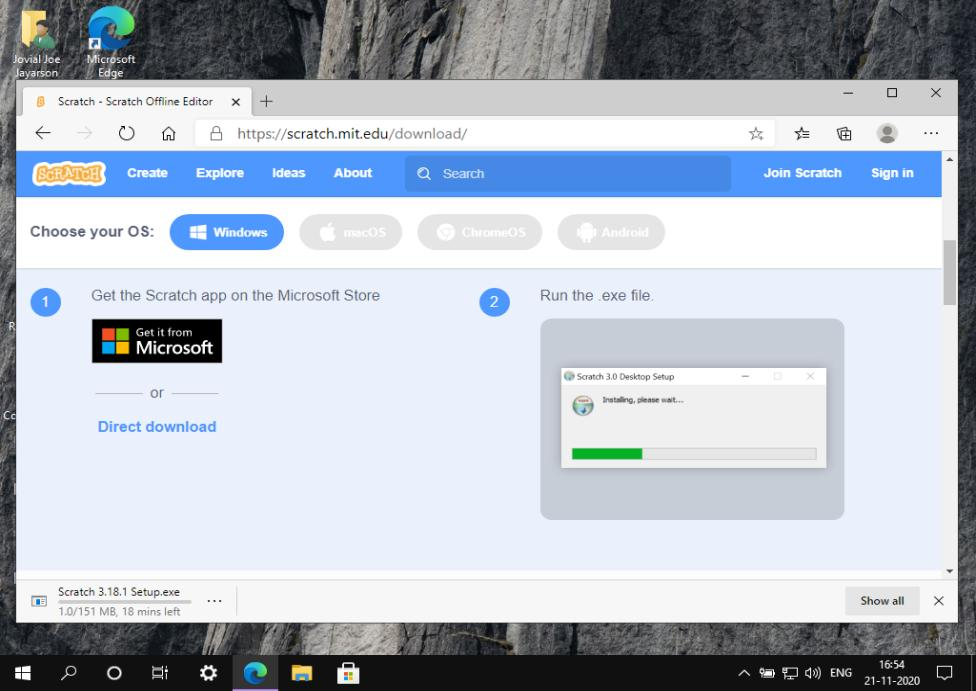
\includegraphics[width = .8\linewidth]{01}
    \end{figure}
    \item Open any browser and goto \href{https://scratch.mit.edu/download}{https://scratch.mit.edu/download}.
    \item Click on \textbf{Direct download}.
    \item Wait for the file to download (it's huge!). Once completed click on the Scratch installer.

          \begin{figure}[H]
              \centering
              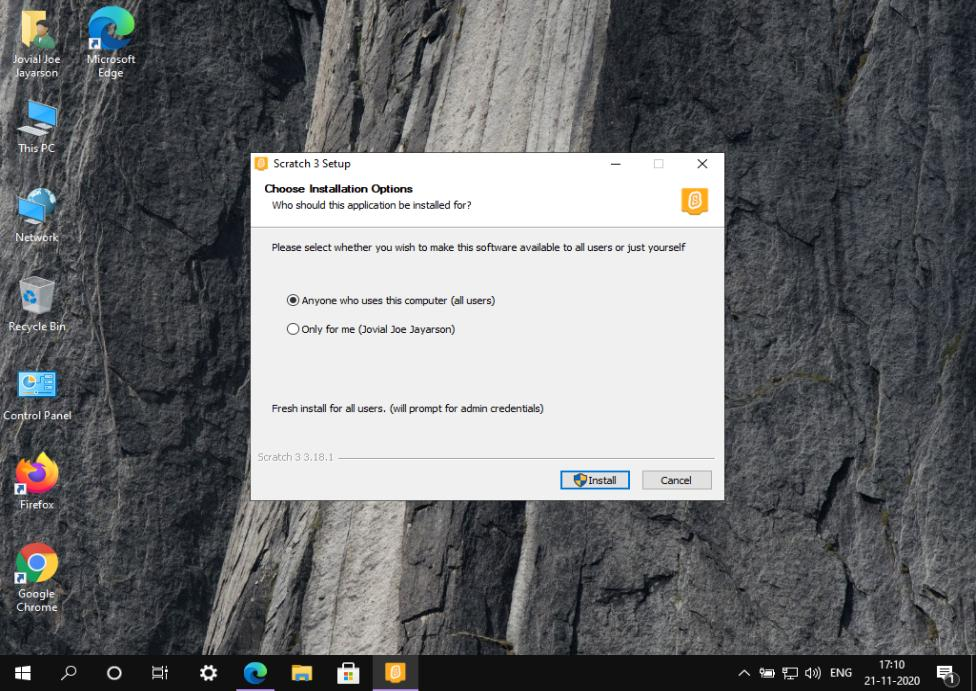
\includegraphics[width = .8\linewidth]{02}
          \end{figure}

    \item Click on \textbf{Install}.

          \begin{figure}[H]
              \centering
              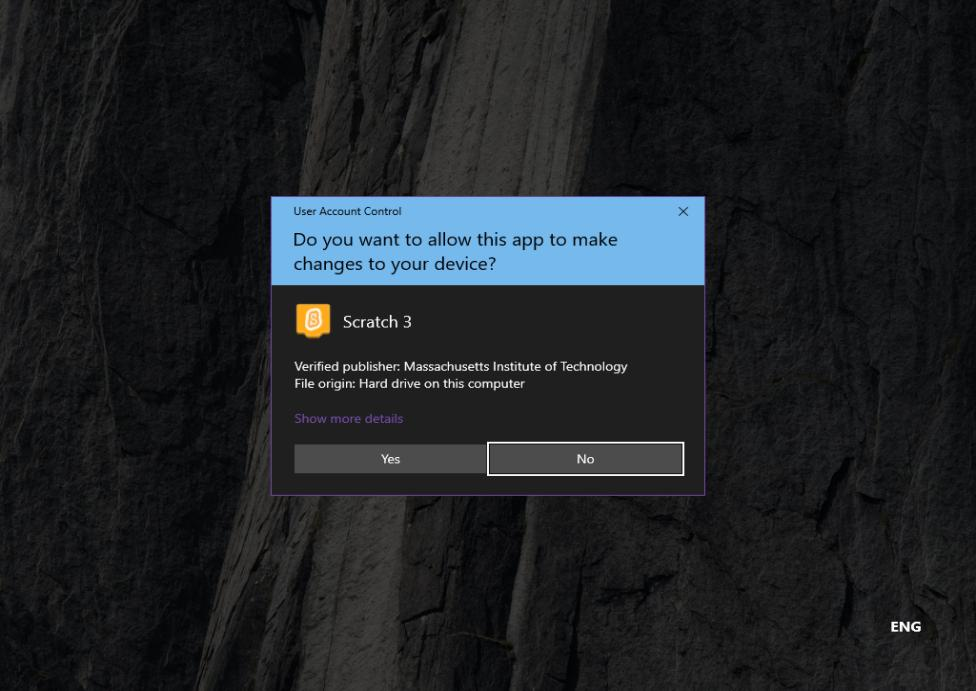
\includegraphics[width = .8\linewidth]{03}
          \end{figure}

    \item Click on \textbf{Yes}.

          \begin{figure}[H]
              \centering
              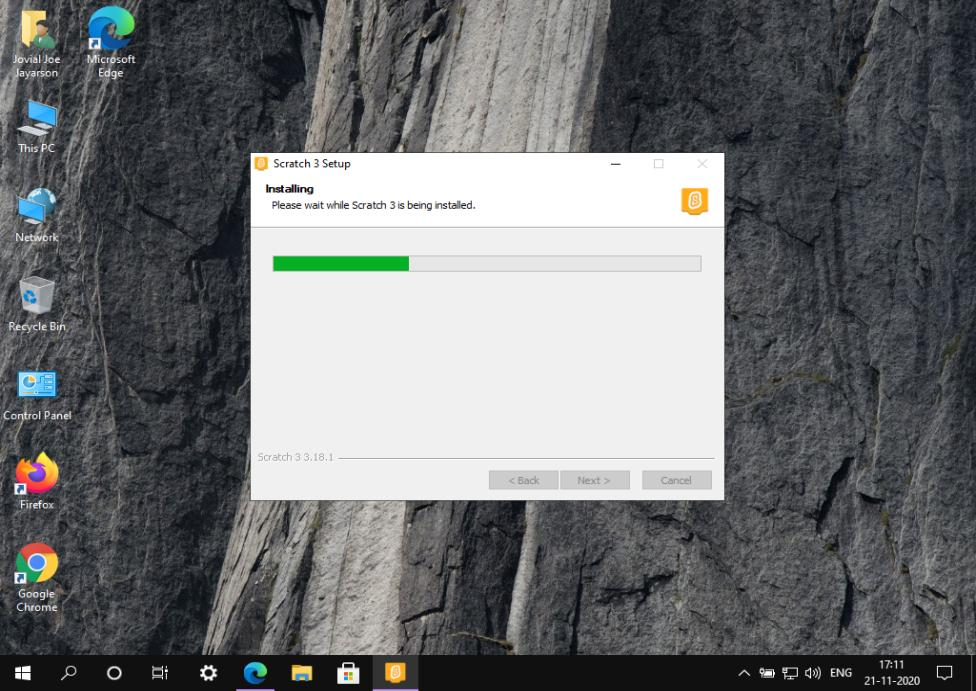
\includegraphics[width = .8\linewidth]{04}
          \end{figure}

    \item Wait for the program to finish installing.

          \begin{figure}[H]
              \centering
              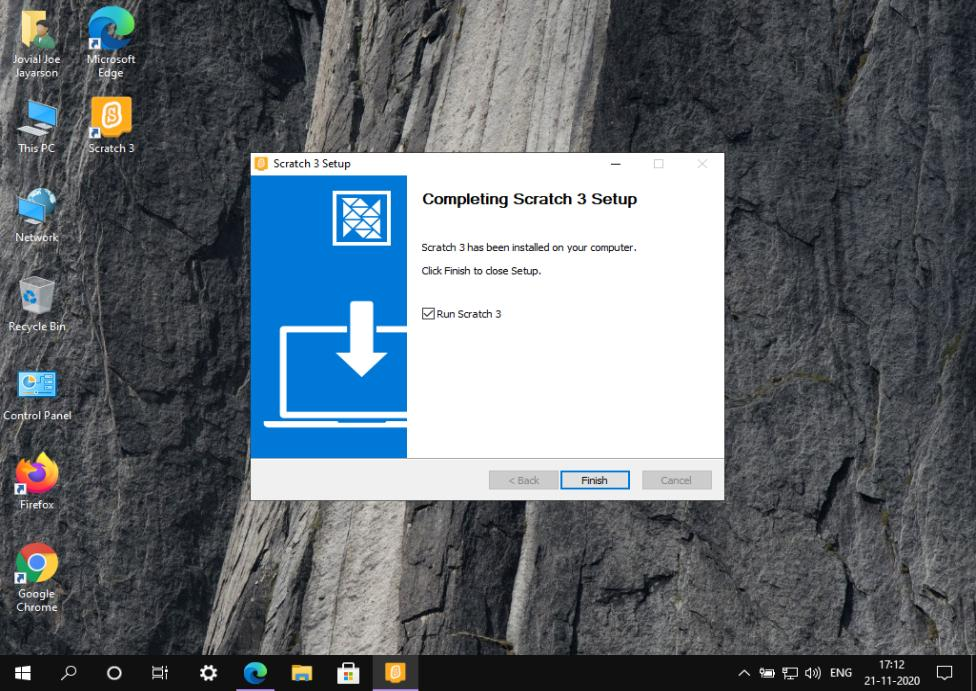
\includegraphics[width = .8\linewidth]{05}
          \end{figure}

    \item Click \textbf{Finish}.

          \begin{figure}[H]
              \centering
              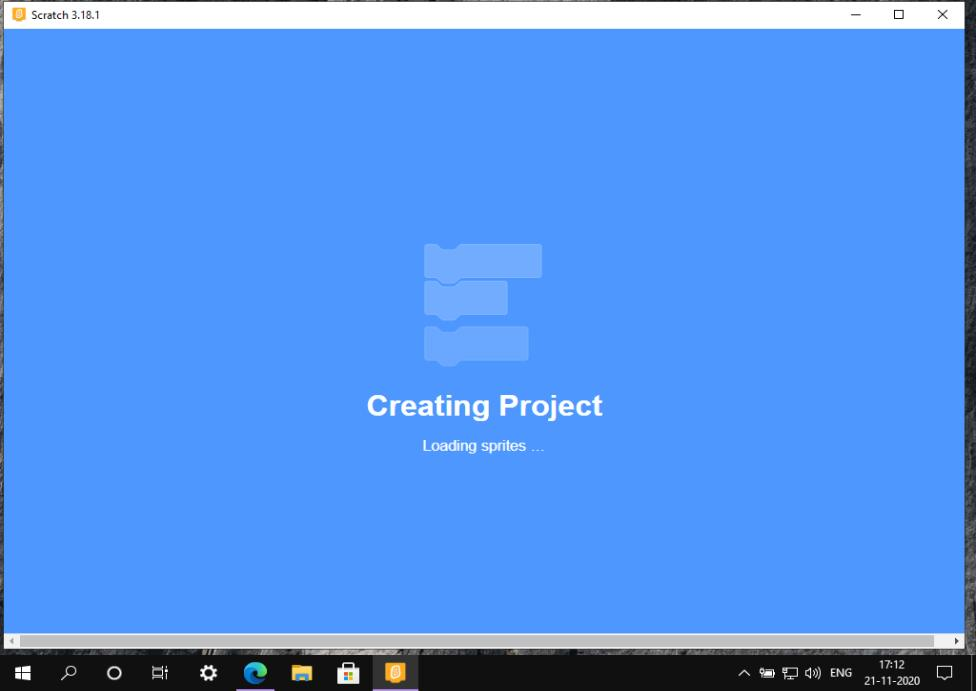
\includegraphics[width = .8\linewidth]{06}
          \end{figure}

    \item Let the Scratch application load.

          \begin{figure}[H]
              \centering
              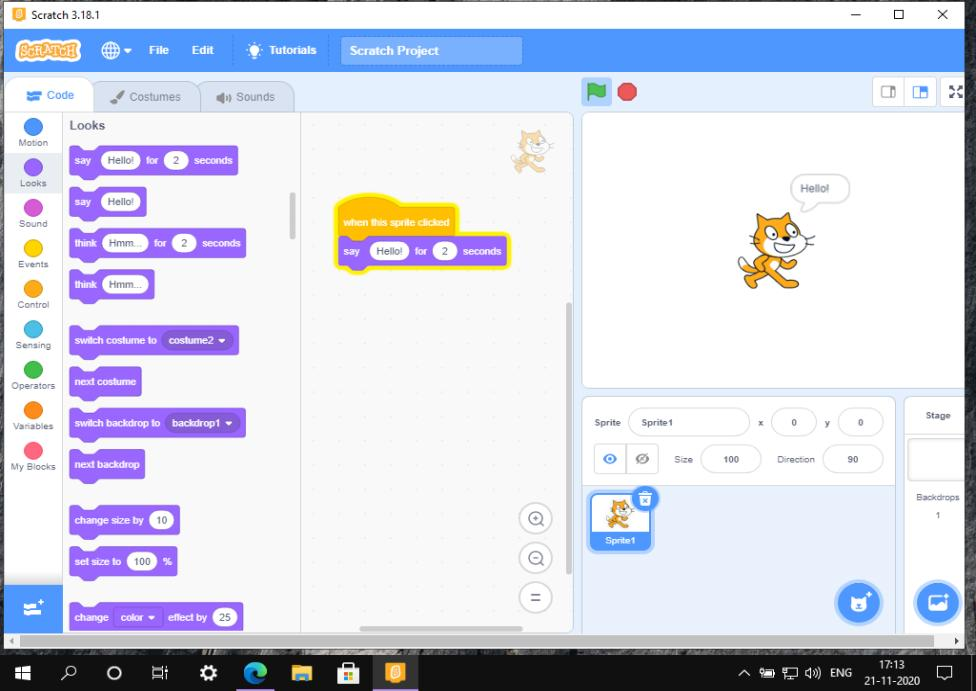
\includegraphics[width = .8\linewidth]{07}
          \end{figure}

    \item Work on your project.

          \begin{figure}[H]
              \centering
              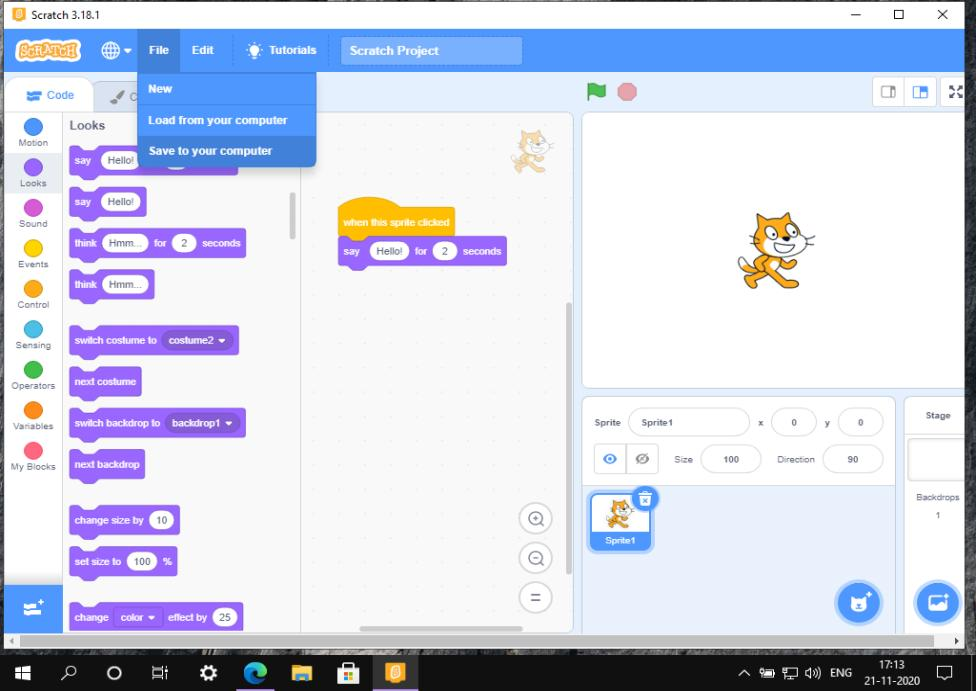
\includegraphics[width = .8\linewidth]{08}
          \end{figure}

    \item Click on \textbf{File} then click \textbf{Save to your computer}.

          \begin{figure}[H]
              \centering
              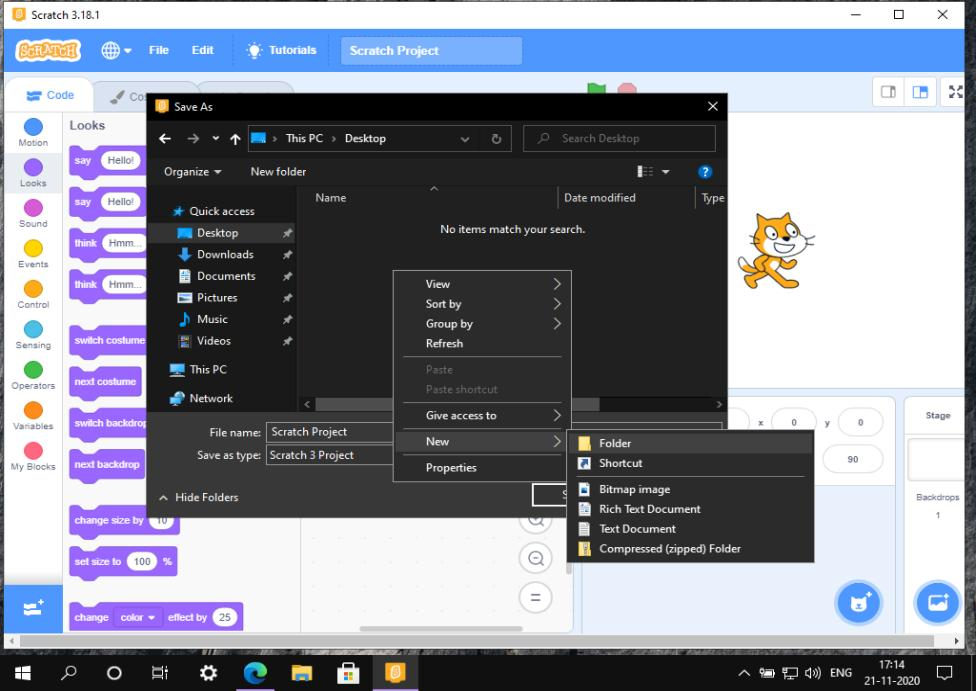
\includegraphics[width = .8\linewidth]{09}
          \end{figure}

          \begin{figure}[H]
              \centering
              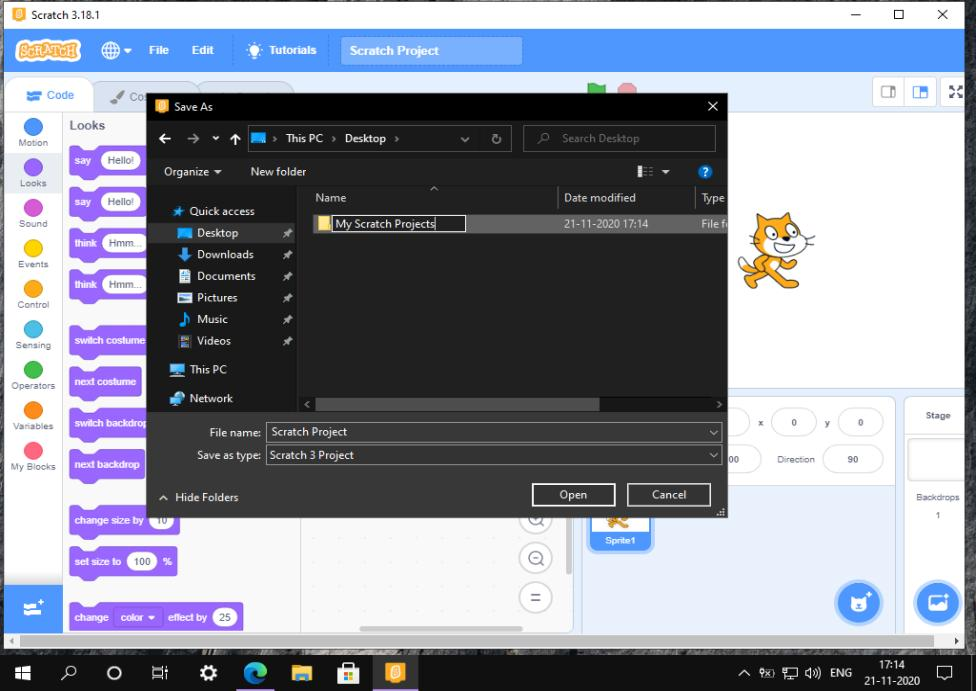
\includegraphics[width = .8\linewidth]{10}
          \end{figure}

    \item Create a folder and name it \textit{My Scratch Projects}. Remember the location of the folder.

          \begin{figure}[H]
              \centering
              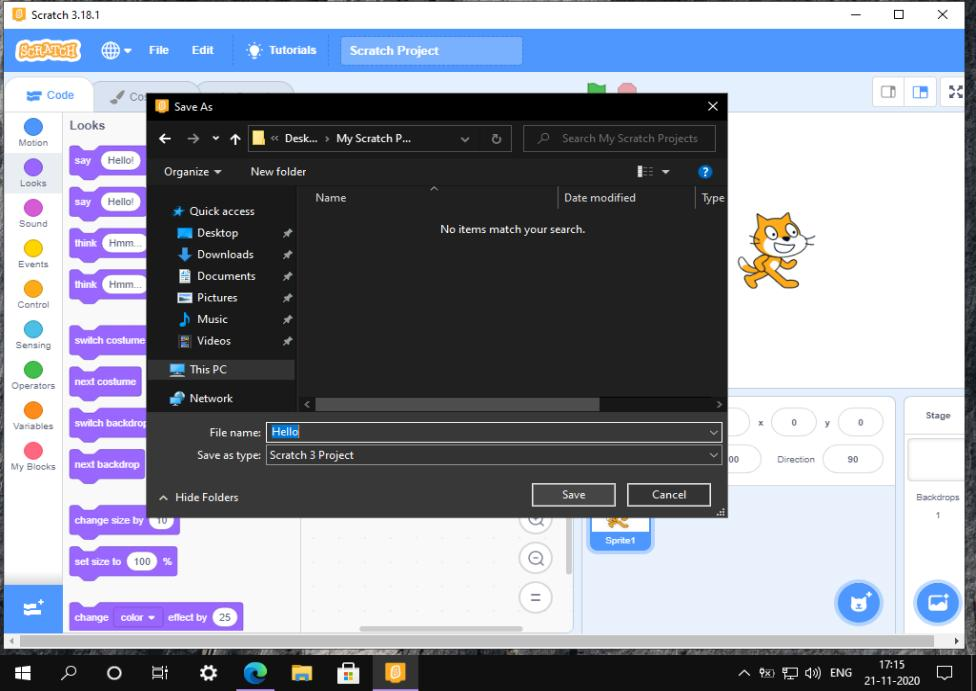
\includegraphics[width = .8\linewidth]{11}
          \end{figure}

    \item Name the file to suit your project.

          \begin{figure}[H]
              \centering
              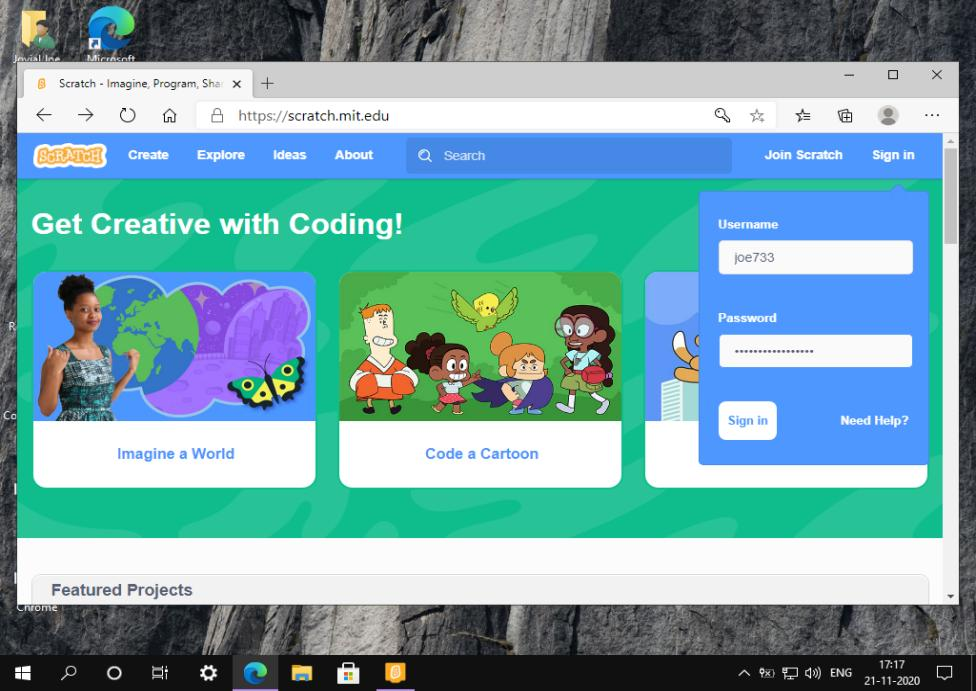
\includegraphics[width = .8\linewidth]{12}
          \end{figure}

    \item Open browser head onto: \href{https://scratch.mit.edu/}{https://scratch.mit.edu/}.
    \item Click \textbf{Sign in}. Enter your \textit{username} and \textit{password}. Click the white \textbf{Sign in} button.

          \begin{figure}[H]
              \centering
              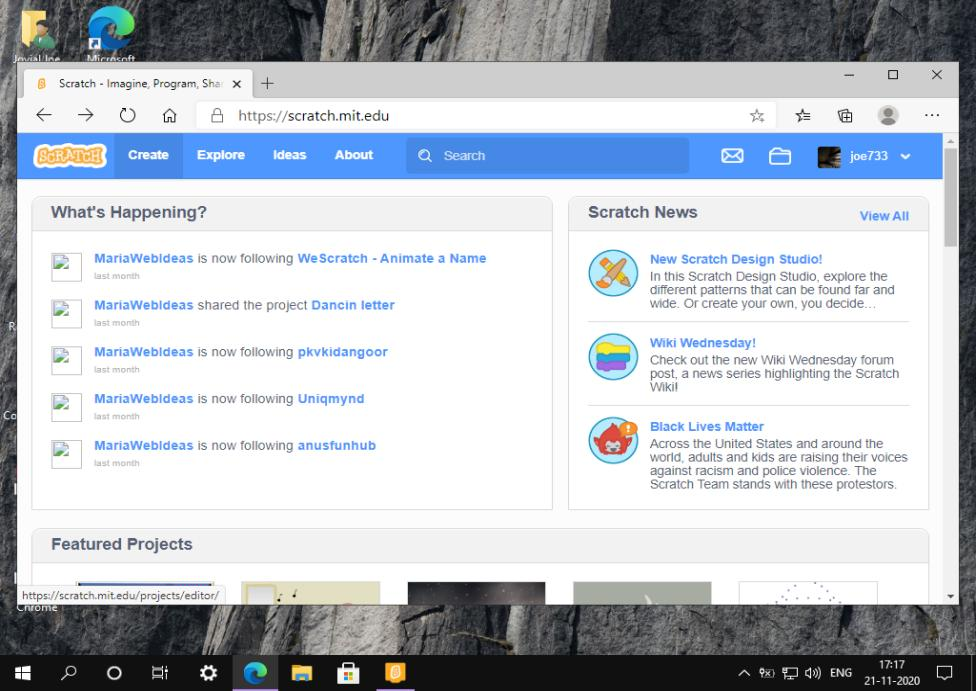
\includegraphics[width = .8\linewidth]{13}
          \end{figure}

    \item Once your logged in, click on \textbf{Create}.

          \begin{figure}[H]
              \centering
              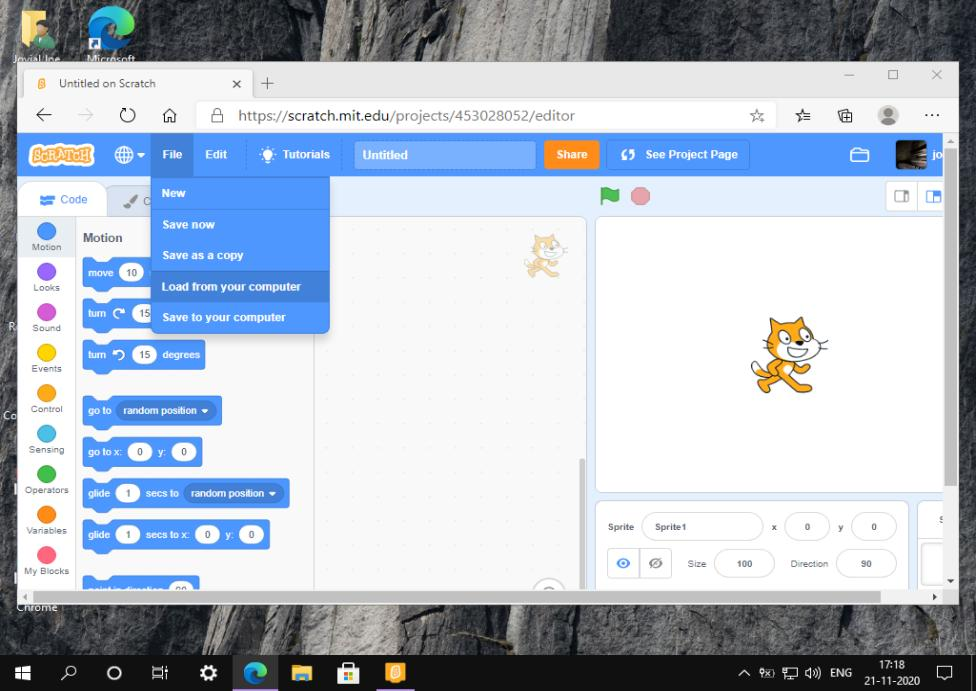
\includegraphics[width = .8\linewidth]{14}
          \end{figure}

    \item After your scratch project loads up, click on \textbf{File} and select \textbf{Load from your computer} in the drop-down menu.

          \begin{figure}[H]
              \centering
              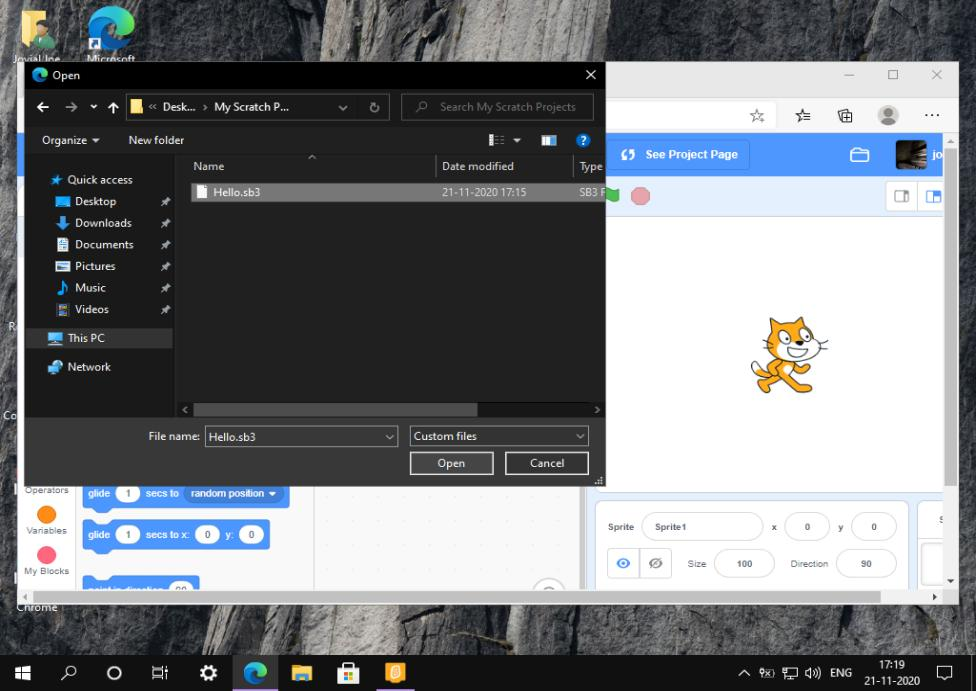
\includegraphics[width = .8\linewidth]{15}
          \end{figure}

    \item Locate your file, and click \textbf{Open}.

          \begin{figure}[H]
              \centering
              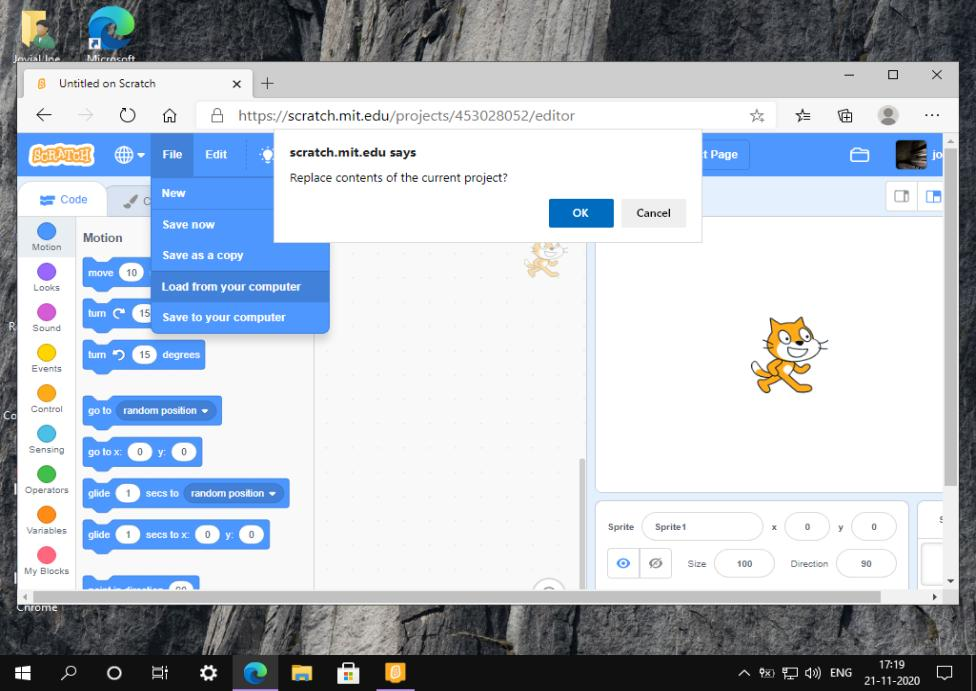
\includegraphics[width = .8\linewidth]{16}
          \end{figure}

    \item If an alert box pops up, click \textbf{Ok}.

          \begin{figure}[H]
              \centering
              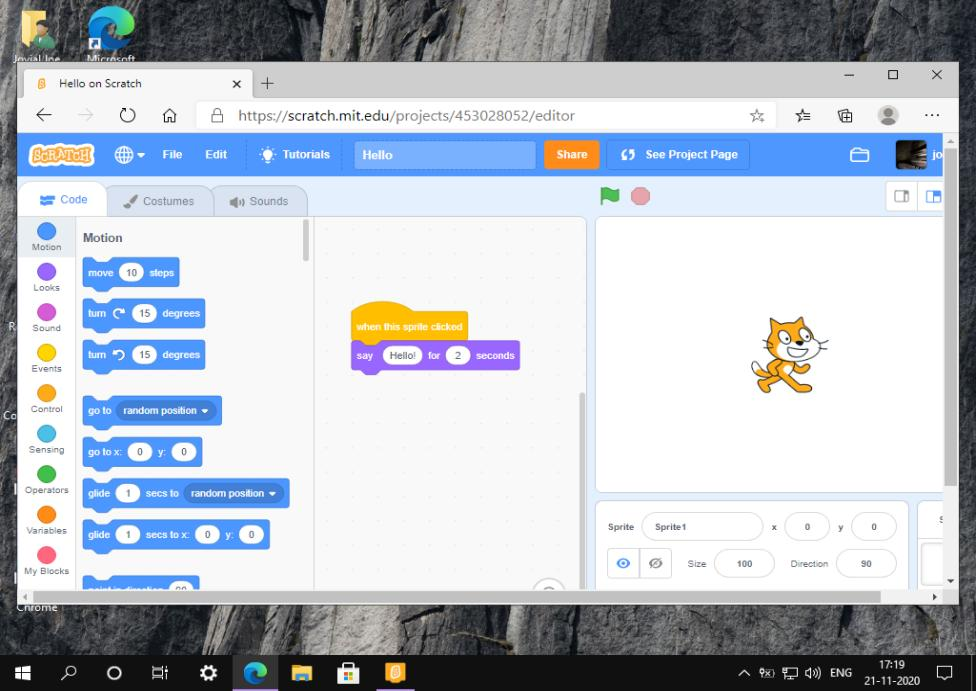
\includegraphics[width = .8\linewidth]{17}
          \end{figure}

    \item There you go. You have uploaded your scratch project to your account. Smash the bright orange \textbf{Share} button.

          \begin{figure}[H]
              \centering
              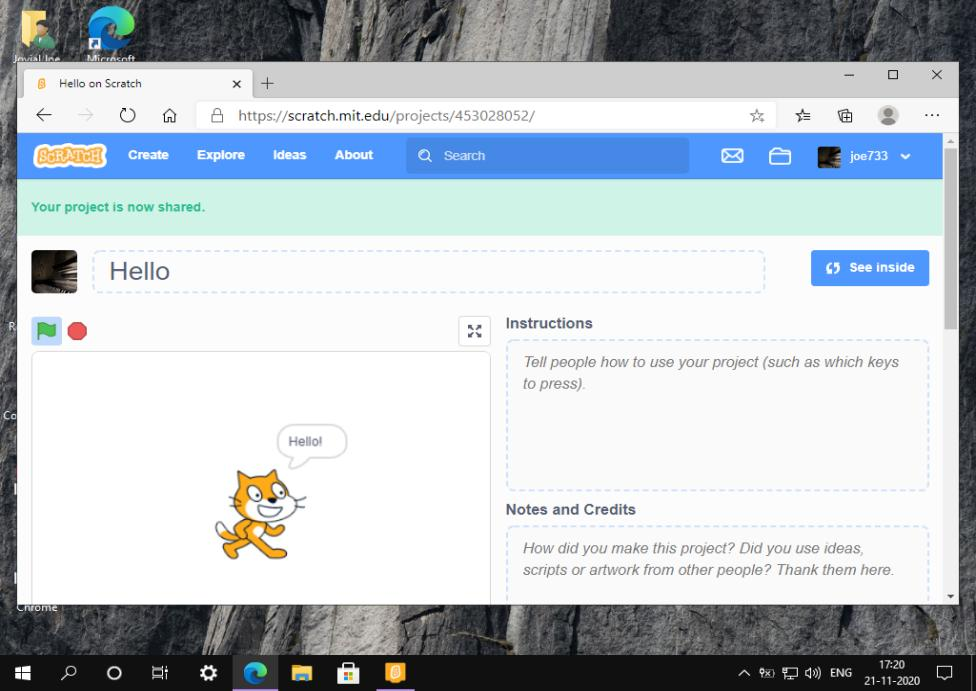
\includegraphics[width = .8\linewidth]{18}
          \end{figure}

    \item Bingo! The whole world can see your project.
\end{enumerate}
\vspace{1cm}
\begin{center}
    \textbf{Tip:} \textit{It's recommended to use Scratch right from your browser. It will avoid much hassle.}
\end{center}
\end{document}